\documentclass[14]{article}

% Used packages
\usepackage{apacite}
\usepackage[12pt]{moresize}
%\usepackage[numbers,sort&compress]{natbib}
\usepackage{blindtext}
\usepackage{enumitem}
\usepackage{xcolor}
\usepackage[explicit,noindentafter]{titlesec}
\usepackage[rightcaption]{sidecap}
\usepackage{caption}
\usepackage{float}
\usepackage{csquotes}
\usepackage{titling}
\usepackage{titlesec}
\usepackage{graphicx} %package to manage images
\graphicspath{{images/}}



\titlespacing\section{1pt}{12pt plus 0pt minus 0pt}{6pt plus 0pt minus 0pt}
\titlespacing\subsection{1pt}{12pt plus 4pt minus 2pt}{6pt plus 2pt minus 2pt}
\titlespacing\subsubsection{1pt}{12pt plus 4pt minus 2pt}{6pt plus 2pt minus 2pt}
\titlespacing\paragraph{1pt}{12pt plus 4pt minus 2pt}{6pt plus 2pt minus 2pt}

% New commands
\newcommand{\addsection}[3]{\addtocontents{toc}{\protect\contentsline{section}{\protect\numberline{#1}#2}{#3}}}
\newcommand{\addsubsection}[3]{\addtocontents{toc}{\protect\contentsline{subsection}{\protect\numberline{#1}#2}{#3}}}
\newcommand{\itab}[1]{\hspace{0em}\rlap{#1}}
\newcommand{\tab}[1]{\hspace{.5\textwidth}\rlap{#1}}
\newcommand{\Csh}{C{\lserif\#}}


\begin{document}
\author{\textbf{Faculty of Sciences and Bio-Engineering Sciences}\\[2\baselineskip]\newline\textbf{Arthur Chomé - 0529279}}

\date{ \LARGE Assignment 2: Statistics}
\title{\vspace{-8cm}}%\underline{Everything is connected}}

\maketitle

\section{Introduction}
As a second assignment for the course Methods for Scientific Research, we have to fulfil four statistical exercises. Further details of which can be found in the assignment document available on Canvas. Also provided were the datasets to be used for the exercises, based on our student number (0529279) the set number calculator\footnote{\protect\url{https://ai.vub.ac.be/~bart/statsnumbers.html}} assigned us with the sets 4, 1, 4, 3 for the four respective questions. All tests, charts and diagrams were generated using IBM's SPSS Statistics package version 23\footnote{\protect\url{https://en.wikipedia.org/wiki/SPSS}} released in 2015. 

\section{Question 1}
The used dataset --set 4 for the first question-- was gathered by way of an experiment measuring the resonance frequencies of two types of crystal oscillators (variables x1 and x2) needed to provide timing information for high performance hardware. 

\subsection{Diagram}
The use of boxplots is a standardized way of displaying the distribution of data based various L-estimators such as the minimum, first quartile, median, third quartile and maximum.

\begin{figure}[!htb]
	\includegraphics[width=1.0\textwidth]{img/question1/Question1_Boxplot.PNG}
	\captionsetup{width=1.0\textwidth}
	\centering
	%\caption{Given boxplots show that both variables have an evenly distributed range. Dataset x1 however has a wider distribution of its data with the maximum and minimum of the data being further away from the median than in dataset x2. } 
\end{figure}
\mbox{}\\ Given boxplots show that both variables have an evenly distributed range. Dataset x1 however has a wider distribution of its data with the maximum and minimum of the data being further away from the median than in dataset x2. 

\paragraph{Explanation}\mbox{}\newline
The use of boxplots is a standardized way of displaying the distribution of data based on the five number summary: minimum, first quartile, median, third quartile, and maximum. Between the first and third quartile lies 50 percent of all data with the median being the middle value of the whole set. Between the maximum and minimum lies about 99.75 percent of all data. Outliers are even further away of the median than the minimum and maximum and represent 0.25 percent of all data.
\newline 
Using boxplots gives us a simple way of detecting certain characteristics of our data such as symmetry and distribution. It summarises our datasets in terms of median, first quartile, third quartile, maximum and minimum and eases comparison between the two.  

\subsection{Welch's T-test}
Based on the experiment's description, we want to see if the same variable applied on two different populations (e.g. different groups of oscillator crystals) makes for a difference of the means of variables. Because the variance of both datasets differs significantly, a normal T-test would not be reliable in doing so. 
\newline
This is why we settle for Welch's T-test because it is robust even when the sample size or the variance is unequal. In this case, an independent T-test is the best option. Our null hypothesis in this case is that the means of both data collections do not differ. 

\begin{figure}[!htb]
	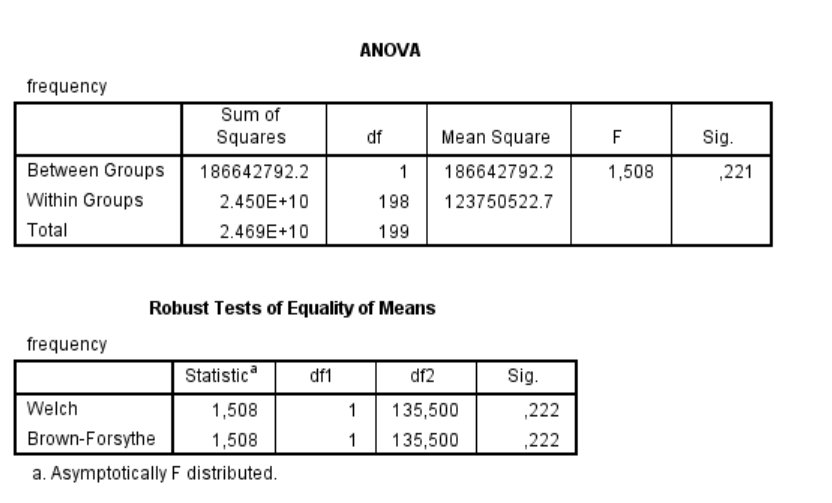
\includegraphics[width=1.0\textwidth]{img/question1/question1_b.PNG}
	\captionsetup{width=1.0\textwidth}
	\centering
	%\caption{Given boxplots show that both variables have an evenly distributed range. Dataset x1 however has a wider distribution of its data with the maximum and minimum of the data being further away from the median than in dataset x2. } 
\end{figure}
\mbox{}\\ 
Because the p-value in this case is greater than 0.05 begin 0.222, we cannot conclude that a significant difference exists and we accept our nullhypothesis.

\subsection{Crystal reliability}
Because both dataset means do not differ significantly and are normally distributed, we can trust both crystal types x1 and x2. 

\section{Question 2}
\section{Question 3}
\section{Question 4}

\end{document}